\subsubsection{User Story}
Những người đứng đầu của hệ thống chia sẻ nhà muốn hệ thống của mình cho phép một số đối tượng nhất định trong hệ thống có thể tạo ra các đợt khuyến mại để thu hút người dùng. Dịch vụ chia sẻ nhà sẽ có 2 loại khuyến mại khác nhau:
\begin{itemize}
	\item  \textbf{Khuyến mãi của hệ thống}: Đây là những khuyến mãi của hệ thống, được tạo ra bởi những quản lí của hệ thống, hay nói các khác đây là những đợt khuyến mãi được áp dụng cho nhiều homestay khác nhau, thuộc nhiều chủ nhà khác nhau. Những khuyến mãi dạng này sẽ do hệ thống quản lí, chi phí sẽ do hệ thống chi trả phí khuyến mãi.
	\item \textbf{Khuyến mãi của chủ nhà dành cho homestay của mình}: Đây là những khuyến mãi của chủ nhà dành cho homestay của mình. Những khuyến mại dạng này được chủ nhà có thể tạo ra bất cứ lúc nào và chỉ áp dụng cho những homestay mà thuộc về chủ nhà đó. Một cách khác, nếu một người không sở hữu bất kì căn nhà nào trong hệ thống thì không thể tạo ra loại khuyến mại này.
\end{itemize}
Chức năng này cho phép những đối tượng của hệ thống như: quản lí hệ thống, các chủ nhà tạo ra các khuyến mại, chỉnh sửa khuyến mại, xóa khuyến mại, quản lí danh sách các khuyến mại của mình.
Một khuyến mại trong hệ thống có thể có nhữn trạng thái sau:
\begin{itemize}
	\item \textit{Đã kết thúc}: Những khuyến mại đã xảy ra và đã kết thúc.
	\item \textit{Đang diễn ra}: Những khuyến mại đang diễn ra.
	\item \textit{Trong tương lai}: Những khuyến mãi sẽ xảy ra trong tương lai.
\end{itemize}
Khi tạo khuyến mại, quản lí hay chủ nhà cần cung cấp các thông tin như: 
\begin{itemize}
	\item \textit{Tên đợt khuyến mại} 
	\item \textit{Logo của khuyến mại (nếu có)}
	\item \textit{Mô tả khuyến mại}
	\item \textit{Phạm vi áp dụng} 
	\item \textit{Giá trị} 
	\item \textit{Một số thông tin khác(nếu có)}
\end{itemize}
\subsubsection{Các usecase chi tiết}
\begin{figure}[!h]
	\centering
	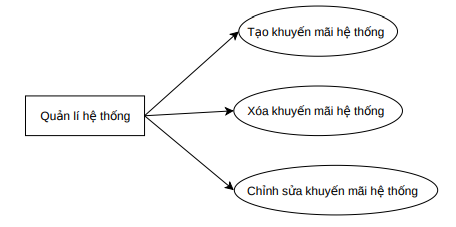
\includegraphics[width=10cm]{Image/module2aa.png}
	\vspace{0.5cm}
	\caption{Lược đồ use case của Module 2: Quản lí khuyến mại (Dành cho quản lí hệ thống}
\end{figure}
\begin{figure}[!h]
	\centering
	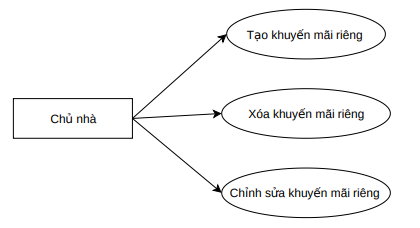
\includegraphics[width=10cm]{Image/module2b.png}
	\vspace{0.5cm}
	\caption{Lược đồ use case của Module 2: Quản lí khuyến mại (Dành cho chủ nhà)}
\end{figure}
\newpage 
\subsubsubsection{Usecase 2: Thêm khuyến mại của hệ thống}
\begin{figure}[!h]
	\centering
	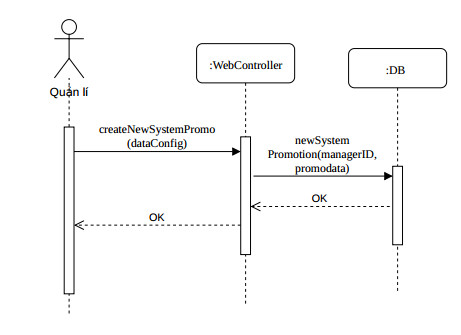
\includegraphics[width=10cm]{Image/createSystemPromoSequence.png}
	\caption{Sequence Diagram cho usecase Thêm khuyến mại hệ thống}
\end{figure}
\begin{center}
	\begin{longtable}{ | l |p{10cm}|}
		\hline
		\textbf{Tên usecase} & Thêm khuyến mại của hệ thống \\ \hline
		\textbf{Người tương tác} & Quản lí hệ thống \\ \hline   
		\textbf{Mô tả} & Cho phép thêm một sự kiện khuyến mãi được áp dụng cho nhiều homestay của các chủ nhà khác nhau cùng một lúc. Khuyến mãi này là của hệ thống, cần phân biệt khuyến mãi này với khuyến mãi của chủ nhà dành cho nhà của mình. \\ \hline  
		\textbf{Người tạo:} \textit{Đinh Minh Tân} & \textbf{Cập nhật lần cuối bởi:} \textit{Đinh Minh Tân} \\ \hline
		\textbf{Ngày tạo:} \textit{22/03/2019} & \textbf{Lần cuối cập nhật:} \textit{30/03/2019} \\ \hline
		\textbf{Tiền điều kiện} & Người dùng đã đăng nhập vào hệ thống bằng quyền của người quản lí, người dùng đang ở màn hình index của trang web.  \\ \hline 
		\textbf{Hậu điều kiện} & Người quản lí quay về màn hình quản lí khuyến mại. \\ \hline 
		\textbf{Luồng cơ bản} & 
		\begin{enumerate}
			\item Quản lí nhấn tab Quản lí khuyến mại.
			\item Hệ thống hiển thị danh sách các sự kiện khuyến mại. Danh sách này phân thành 3 tab: Đã kết thúc, Đang diễn ra, Trong tương lai tương ứng với trạng thái của các khuyến mại.
			\item Quản lí chọn button Thêm khuyến mại mới 
			\item Hệ thống hiện thị lên form thông tin để quản lí điền, bao gồm: loại khuyến mại, tên khuyến mại, mô tả, logo, ngày bắt đầu, ngày kết thúc, điều kiện áp dụng ....
			\item Quản lí hoàn thành form và nhấn OK để xác nhận việc tạo khuyến mại này.
			\item Hệ thống thông báo đã tạo khuyến mại thành công.
			\item Hệ thống quay đưa quản lí về tab quản lí khuyến mại.
		\end{enumerate} \\ \hline 
		\textbf{Luồng thay thế} & 
		\begin{itemize} 
			\item \textit{Luồng thay thế 1}
			\begin{enumerate}
				\item Tại bước 2: Nếu không có khuyến mại nào được tìm thấy thì hệ thống in ra dòng chữ "Chưa có khuyến mại nào!" tại mỗi tab như trên.
				\item Luồng tiếp tục tại bước 3. 
			\end{enumerate}
			
			\item \textit{Luồng thay thế 2}
			\begin{enumerate}
				\item Tại bước 2: Nếu việc tạo khuyến mại không thành công thì hệ thống đưa ra thông báo việc tạo khuyến mại thất bại.
				\item Luồng tiếp tục tại bước 7. 
			\end{enumerate}
		\end{itemize} \\ \hline 
		\textbf{Ngoại lệ}  & Không có \\
		\hline
	\end{longtable}
\end{center}
\newpage 
\subsubsubsection{Usecase 3: Thêm khuyến mại riêng (dành cho chủ nhà)}
\begin{figure}[!h]
	\centering
	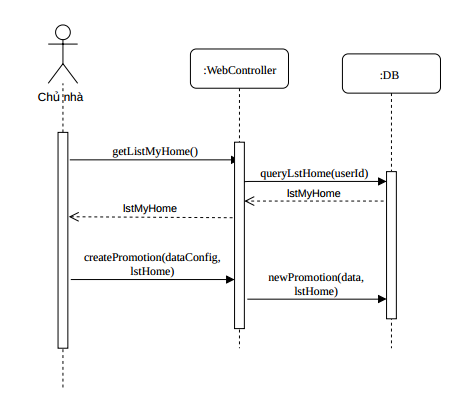
\includegraphics[width=10cm]{Image/createChuNhaPromo.png}
	\caption{Sequence Diagram cho usecase Thêm khuyến mại riêng (dành cho chủ nhà)}
\end{figure}
\begin{center}
	\begin{longtable}{ | l |p{10cm}|}
		\hline
		\textbf{Tên usecase} & Thêm khuyến mại riêng (dành cho chủ nhà) \\ \hline
		\textbf{Người tương tác} & Chủ nhà \\ \hline   
		\textbf{Mô tả} & Cho phép chủ nhà thêm một khuyến mại cho những homestay của mình. \\ \hline  
		\textbf{Người tạo:} \textit{Đinh Minh Tân} & \textbf{Cập nhật lần cuối bởi:} \textit{Đinh Minh Tân} \\ \hline
		\textbf{Ngày tạo:} \textit{22/03/2019} & \textbf{Lần cuối cập nhật:} \textit{30/03/2019} \\ \hline
		\textbf{Tiền điều kiện} & Người dùng đã đăng nhập vào hệ thống với vai trò chủ nhà.  \\ \hline 
		\textbf{Hậu điều kiện} & Chủ nhà quay về màn hình Quản lí khuyến mại. \\ \hline 
		\textbf{Luồng cơ bản} & 
		\begin{enumerate}
			\item Chủ nhà nhấn tab Khuyến mại.
			\item Hệ thống hiển thị danh sách khuyến mại mà chủ nhà đã tạo. Danh sách này phân thành 3 tab: Đã kết thúc, Đang diễn ra, Trong tương lai tương ứng với trạng thái của các khuyến mại.
			\item Chủ nhà chọn button Thêm khuyến mại mới 
			\item Hệ thống hiện lên listbox bao gồm danh sách các homestay mà chủ nhà đang có trên hệ thống
			\item Chủ nhà chọn những homestay mà mình muốn áp dụng khuyến mại trong danh sách trên.
			\item Sau khi chọn homestay xong, chủ nhà nhấn button Tiếp tục để đi đến bước tiếp theo.
			\item Hệ thống hiển thị lên form thông tin để chủ nhà điền, bao gồm: loại khuyến mại, tên khuyến mại, mô tả, logo, ngày bắt đầu, ngày kết thúc, giá trị....
			\item Sau khi hoàn thành form, chủ nhà nhấn OK để Xác nhận tạo khuyến mại.
			\item Hệ thống thông báo đã tạo khuyến mại thành công.
			\item Hệ thống quay đưa chủ nhà về tab Khuyến mại.
		\end{enumerate} \\ \hline 
		\textbf{Luồng thay thế} & 
		\begin{itemize} 
			\item \textit{Luồng thay thế 1}
			\begin{enumerate}
				\item Tại bước 2: Nếu không có khuyến mại nào được tìm thấy thì hệ thống in ra dòng chữ "Chưa có khuyến mại nào!" tại mỗi tab như trên.
				\item Luồng tiếp tục tại bước 3. 
			\end{enumerate}
			
			\item \textit{Luồng thay thế 2}
			\begin{enumerate}
				\item Tại bước 4: Nếu chủ nhà hiện tại không có nhà nào được đăng lên trang web của hệ thống thì hệ thống đưa ra thông báo "Bạn không có nhà nào hiện đang hợp lệ để có thể tạo khuyến mại!"
				\item Tiếp tục tại bước 10 
			\end{enumerate}
			
			\item \textit{Luồng thay thế 3}
			\begin{enumerate}
				\item Tại bước 9: Nếu việc tạo khuyến mại không thành công thì hệ thống đưa ra thông báo việc tạo khuyến mại thất bại.
				\item Luồng tiếp tục tại bước 10. 
			\end{enumerate}
		\end{itemize} \\ \hline 
		\textbf{Ngoại lệ}  & Không có \\
		\hline
	\end{longtable}
\end{center}
\newpage 
\subsubsubsection{Usecase 4: Xóa khuyến mại (dành cho chủ nhà)}
\begin{figure}[!h]
	\centering
	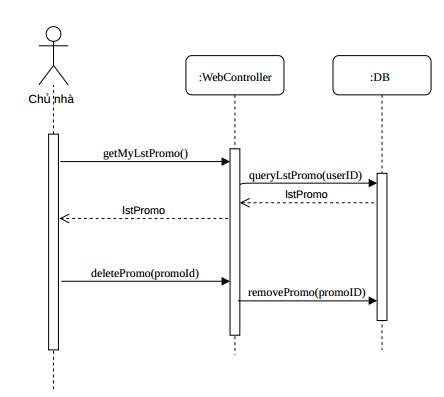
\includegraphics[width=10cm]{Image/deleteChuNhaPromo.png}
	\caption{Sequence Diagram cho usecase Xóa khuyến mại (dành cho chủ nhà)}
\end{figure}
	
\begin{center}
	\begin{longtable}{ | l |p{10cm}|}
		\hline
		\textbf{Tên usecase} & Xóa khuyến mại (dành cho chủ nhà) \\ \hline
		\textbf{Người tương tác} & Chủ nhà \\ \hline   
		\textbf{Mô tả} & Cho phép chủ nhà xóa đi 1 khuyến mại trong danh sách khuyến mại của mình. \\ \hline  
		\textbf{Người tạo:} \textit{Đinh Minh Tân} & \textbf{Cập nhật lần cuối bởi:} \textit{Đinh Minh Tân} \\ \hline
		\textbf{Ngày tạo:} \textit{22/03/2019} & \textbf{Lần cuối cập nhật:} \textit{30/03/2019} \\ \hline
		\textbf{Tiền điều kiện} & Người dùng đã đăng nhập vào hệ thống với vai trò chủ nhà.  \\ \hline 
		\textbf{Hậu điều kiện} & Chủ nhà quay về màn hình Quản lí khuyến mại. \\ \hline 
		\textbf{Luồng cơ bản} & 
		\begin{enumerate}
			\item Chủ nhà nhấn tab Khuyến mại.
			\item Hệ thống hiển thị danh sách khuyến mại mà chủ nhà đã tạo. Danh sách này phân thành 3 tab: Đã kết thúc, Đang diễn ra, Trong tương lai tương ứng với trạng thái của các khuyến mại. Tab Đang diễn ra là tab hiển thị mặc định.
			\item Chủ nhà chọn Tab tương ứng: Đã kết thúc, Đang diễn ra, Trong tương lai để xem danh sách khuyến mại của từng tab.
			\item Chủ nhà chọn khuyến mại mà mình muốn xóa.
			\item Hệ thống hiển thị form xác nhận yêu cầu chủ nhà xác nhận việc xóa khuyến mại này. 
			\item Chủ nhà chọn Xác nhận.
			\item Hệ thống đưa ra thông báo xóa thành công.
			\item Hệ thống quay đưa chủ nhà về tab Khuyến mại.
		\end{enumerate} \\ \hline 
		\textbf{Luồng thay thế} & 
		\begin{itemize} 
			\item \textit{Luồng thay thế 1}
			\begin{enumerate}
				\item Tại bước 2: Nếu không có khuyến mại nào được tìm thấy thì hệ thống in ra dòng chữ "Chưa có khuyến mại nào!" tại mỗi tab như trên.
				\item Luồng tiếp tục tại bước 8. 
			\end{enumerate}
			
			\item \textit{Luồng thay thế 2}
			\begin{enumerate}
				\item Tại bước 3: Nếu tab chủ nhà chọn mà không có khuyến mại nào hiện có thì hiện lên thông báo "Không có khuyến mại nào!"
			\end{enumerate}
			\item \textit{Luồng thay thế 3}
			\begin{enumerate}
				\item Tại bước 6: Tại bước này người dùng chọn "Cancel" để hủy việc xóa khuyến mại.
				\item Luồng tiếp tục tại bước 8. 
			\end{enumerate}
			\item \textit{Luồng thay thế 4}
			\begin{enumerate}
				\item Tại bước 7: Nếu việc xóa khuyến mại không thành công thì hệ thống hiển thị thông báo xóa thất bại.
				\item Luồng tiếp tục tại bước 8. 
			\end{enumerate}
		\end{itemize} \\ \hline 
		\textbf{Ngoại lệ}  & Không có \\
		\hline
	\end{longtable}
\end{center}
	
\subsubsubsection{Usecase 5: Xóa khuyến mại hệ thống (dành cho quản lí)}
\begin{figure}[!h]
	\centering
	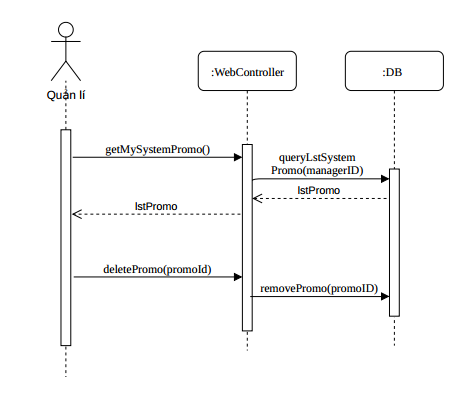
\includegraphics[width=10cm]{Image/deleteSystemPromo.png}
	\caption{Sequence Diagram cho usecase Xóa khuyến mại hệ thống (dành cho quản lí)}
\end{figure}
\begin{center}
	\begin{longtable}{ | l |p{10cm}|}
		\hline
		\textbf{Tên usecase} & Xóa khuyến mại hệ thống (dành cho quản lí) \\ \hline
		\textbf{Người tương tác} & Quản lí hệ thống. \\ \hline   
		\textbf{Mô tả} & Cho phép quản lí xóa đi một sự kiện khuyến mãi của hệ thống. \\ \hline  
		\textbf{Người tạo:} \textit{Đinh Minh Tân} & \textbf{Cập nhật lần cuối bởi:} \textit{Đinh Minh Tân} \\ \hline
		\textbf{Ngày tạo:} \textit{22/03/2019} & \textbf{Lần cuối cập nhật:} \textit{30/03/2019} \\ \hline
		\textbf{Tiền điều kiện} & Người dùng đã đăng nhập vào hệ thống với vai trò quản lí.  \\ \hline 
		\textbf{Hậu điều kiện} & Quản lí quay về màn hình Quản lí khuyến mại. \\ \hline 
		\textbf{Luồng cơ bản} & 
		\begin{enumerate}
			\item Quản lí nhấn tab Quản lí khuyến mại.
			\item Hệ thống hiển thị danh sách khuyến mại mà quản lí đã tạo. Danh sách này phân thành 3 tab: Đã kết thúc, Đang diễn ra, Trong tương lai tương ứng với trạng thái của các khuyến mại. Tab Đang diễn ra là tab hiển thị mặc định.
			\item Quản lí chọn Tab tương ứng: Đã kết thúc, Đang diễn ra, Trong tương lai để xem danh sách khuyến mại của từng tab.
			\item Quản lí chọn khuyến mại mà mình muốn xóa.
			\item Hệ thống hiển thị form xác nhận yêu cầu quản lí xác nhận việc xóa khuyến mại này. 
			\item Quản lí chọn Xác nhận.
			\item Hệ thống đưa ra thông báo xóa thành công.
			\item Hệ thống quay đưa quản lí về tab Quản lí khuyến mại.
		\end{enumerate} \\ \hline 
		\textbf{Luồng thay thế} & 
		\begin{itemize} 
			\item \textit{Luồng thay thế 1}
			\begin{enumerate}
				\item Tại bước 2: Nếu không có khuyến mại nào được tìm thấy thì hệ thống in ra dòng chữ "Chưa có khuyến mại nào!" tại mỗi tab như trên.
				\item Luồng tiếp tục tại bước 8.
			\end{enumerate}
			
			\item \textit{Luồng thay thế 2}
			\begin{enumerate}
				\item Tại bước 3: Nếu tab quản lí chọn mà không có khuyến mại nào hiện có thì hiện lên thông báo "Không có khuyến mại nào!"
			\end{enumerate}
			
			\item \textit{Luồng thay thế 3}
			\begin{enumerate}
				\item Tại bước 6: Tại bước này quản lí chọn "Cancel" để hủy việc xóa khuyến mại.
				\item Luồng tiếp tục tại bước 8. 
			\end{enumerate}
			
			\item \textit{Luồng thay thế 4}
			\begin{enumerate}
				\item Tại bước 7: Nếu việc xóa khuyến mại không thành công thì hệ thống hiển thị thông báo xóa thất bại.
				\item Luồng tiếp tục tại bước 8. 
			\end{enumerate}
		\end{itemize} \\ \hline 
		\textbf{Ngoại lệ}  & Không có \\
		\hline
	\end{longtable}
\end{center}